\documentclass[16pt,answers]{exam}
\author{Nima Poshtiban}
\title{Digital Electronics}
\usepackage{datetime}
\newdate{date}{26}{10}{2025}
\newdate{due}{1}{11}{2025}
\date{\displaydate{date}}
\usepackage[utf8]{inputenc}
\usepackage{amsmath}
\usepackage{enumitem}
\usepackage{graphicx}
\usepackage[urlcolor=blue, bookmarksopen]{hyperref}
\usepackage[]{geometry}
\usepackage[]{cleveref}
\usepackage{amsmath}
\usepackage{xcolor}
\usepackage{siunitx}
\usepackage{tikz}
\usepackage{svg}
\usepackage{tikz}
\usepackage{circuitikz}
\usepackage{float}
\usepackage[export]{adjustbox}
\begin{document}
\maketitle
\tableofcontents 
\pagebreak

\section{Assignment No.1}
\begin{center}
\fbox{\fbox{\parbox{5.5in}{\centering
Assignment Due: \displaydate{due}}}}
\end{center}


\begin{questions}
	
\question \begin{parts}
	\part Illustrate the evolution of the processors between 1978 to 2018 in terms of Cost, Performance and Power Dissipation.\\
	\linebreak
	\paragraph{}
	It all started with the release of the legendary microprocessor \textbf{Intel 8086}! first a 16bit processors then the start for pushing the architecture to 32bit had began; The new chips made multi-tasking possible.At 80's The competition for evolving processors has already began, and this contributed to processor design evolution, thus leading to the exponential growth in performance. The manufacture Companies kept pushing towards higher frequencies, less area size, and more efficiency. In 2000's the advent of multi-core CPUs created a new phase of competition based on the mentioned factors. But the Moore's law has became the main reason limiting the clock frequency, because with higher clock speed, the higher Temperature is produced and cooling system itself is a big challenge, making the higher speed clocks nigh-impossible. \\
	\part has technology been following any pattern ever since? 
	\\
	\paragraph{}
	Not entirely, but there is somewhat a pattern in the number of transistors per chip which doubles nearly every 10 year (not always true).
	\\
	\part What's your take on the relation between Dennard Scaling, memory wall and power wall?
	\\
	\paragraph{}
	According to Dennard's claim the since 2005's we have reached a dead-lock in clock speed due to direct proportion between frequency and Power Dissipation which introduced the term Power Wall. The similar problems exist for memory size and speed, because memories failed to keep up with the pace of CPU development. Now it's crystal clear that the only option is adding more core instead of pushing for more clock speed, and for memories they are increasing the refresh rate but DDR5 proved to be a challenged itself, while so fast, it will become unstable at 64Gig capacity, causing power leakage and even worse, complete motherboard failures. 
\end{parts}
\question
\begin{parts}
 \part Illustrate the following terms in full details with examples: Propagation delay, Noise Margin, Timing failure and Rising timing
 \\
 \paragraph{}
 \begin{enumerate}
 	\item Propagation Delay: The time span between circuit transition from input to output.
 	meaning \[
 		t_{pd}\,= \frac{1}{2}t_{phl} + \frac{1}{2}t_{plh}  
 	\]
 	for example if it takes 2ns to going from high state to low state and 4ns for the opposite
 	The propagation delay is \[
 		t_{pd}\,=\frac {1}{2}\cdot2+\frac{1}{2}\cdot4 \Longrightarrow t_{pd}=3ns
 	\]
 	\item Timing failure $t_{f}$ and Rising timing $t_{r}$
 	As the name suggests Timing failure is the span of shifting quiescent point towards the low state. Rising Time is the duration of changing from Low state into high state point (which can be the quiescent point). the range of both(often) is from 10 percent to 90 percent of the total transition time for each.
 	\item Noise Margin
 	Is the maximum voltage threshold that can be added to the circuit without causing illegal states. The difference between the tolerance for Input High state and Output high state is called NMH and the inverse of that is called NML  
 	\[
 		NMH =V_{OH} - V_{IH} ,\quad 
 		NML = V_{IL} - V_{OL}
 	\] 
 \end{enumerate}
 \part By Simulating a RC circuit, find the formulas for Propagation Delay\\


\usetikzlibrary{decorations.pathreplacing}   % for curly braces
	
	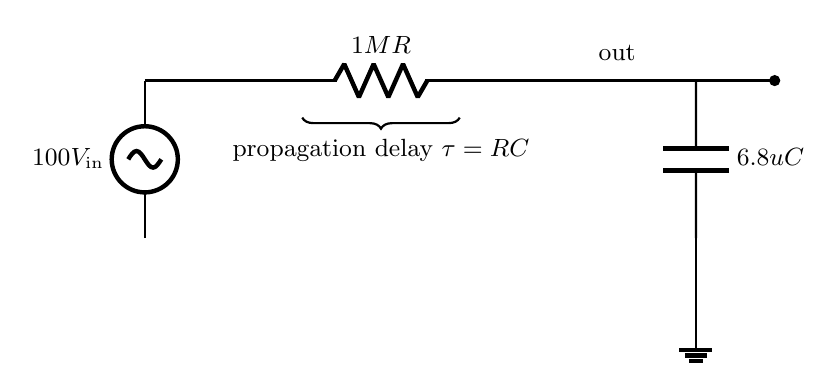
\begin{tikzpicture}[american,
		font=\small,
		thick]
		
		%--- Voltage source (generic) ---------------------------------
		\draw (0,0) to[sV, l=$100V_{\text{in}}$] (0,2);
		
		%--- Resistor -------------------------------------------------
		\draw (0,2) -- (2,2) to[R, l=$1MR$] (4,2);
		\draw (4,2) to[short,-*,l=out] (8,2);
		%--- Capacitor ------------------------------------------------
		\draw (7,2) to[C, l=\({6.8uC}\)] (7,0);
		
		%--- Ground ---------------------------------------------------
		\draw (7,0) -- (7,-1) node[ground] {};
		
		%--- Close the loop -------------------------------------------
		
		
		%--- Propagation-delay annotation (curly brace + label) ------
		\draw[decorate,decoration={brace,amplitude=4pt,mirror,raise=2pt}]
		(2,1.6) -- (4,1.6)
		node[midway,below=6pt] {propagation delay $\tau = RC$};
	
	\end{tikzpicture}	\label{rc}
	\\
	simulation showed 7 thus
	\[
		\tau \approx \,1MR \times\, 6.8\cdot10^{-6}
	\]
\\
\end{parts}
\question\begin{parts}
	\part\textit{ Define the Power Consumption and Energy Consumption in details}
	\\
	Power Consumption means the ratio of Voltage and Current in a definite time, Some write this as \(P\,=v(t)I(t)\) which is totally wrong, I and V \textbf{are not proportional}.
	\\
	Energy Consumption is average Power Consumption of a thing. the formula can be written as \[
		\overline{P}\,=\Re(\oint_{0}^{T}v(t)I(t)dt)
	\]
	\part\textit{ By Simulating a RC circuit, find the formulas for Power} \\
	by using the same circuit ( \ref{rc})\\
	We find that the formula for Power Consumption is approximate one and not right as
	the numbers from previous \textbf{simulation does not add up }
	
\end{parts}
\question\textit{ Elaborate the concept of Digital gate noise immunity}
\\
In a nutshell it can be described as "The ability to withstand unwanted noise and operate correctly". To make this happen the proper routing and placements are crucial factors. Thus wires path must not cross or interfere via an electro-magnetic field. Moreover, the logic level design must prevent this by using extra gates for static-hazard removals.



\question Draw the schematics of an Exclusive OR (XOR) using \textbf{MOSFETs} (\textbf{BJTs are prohibited})
\paragraph{}
\begin{figure}[H]
 	\centering
\includegraphics[scale=0.7]{xor.pdf}
\caption{XOR}

\end{figure}


\question Run the given HDL file and report back the results (Screenshots are Mandatory)
\paragraph{}


\begin{figure}[H]

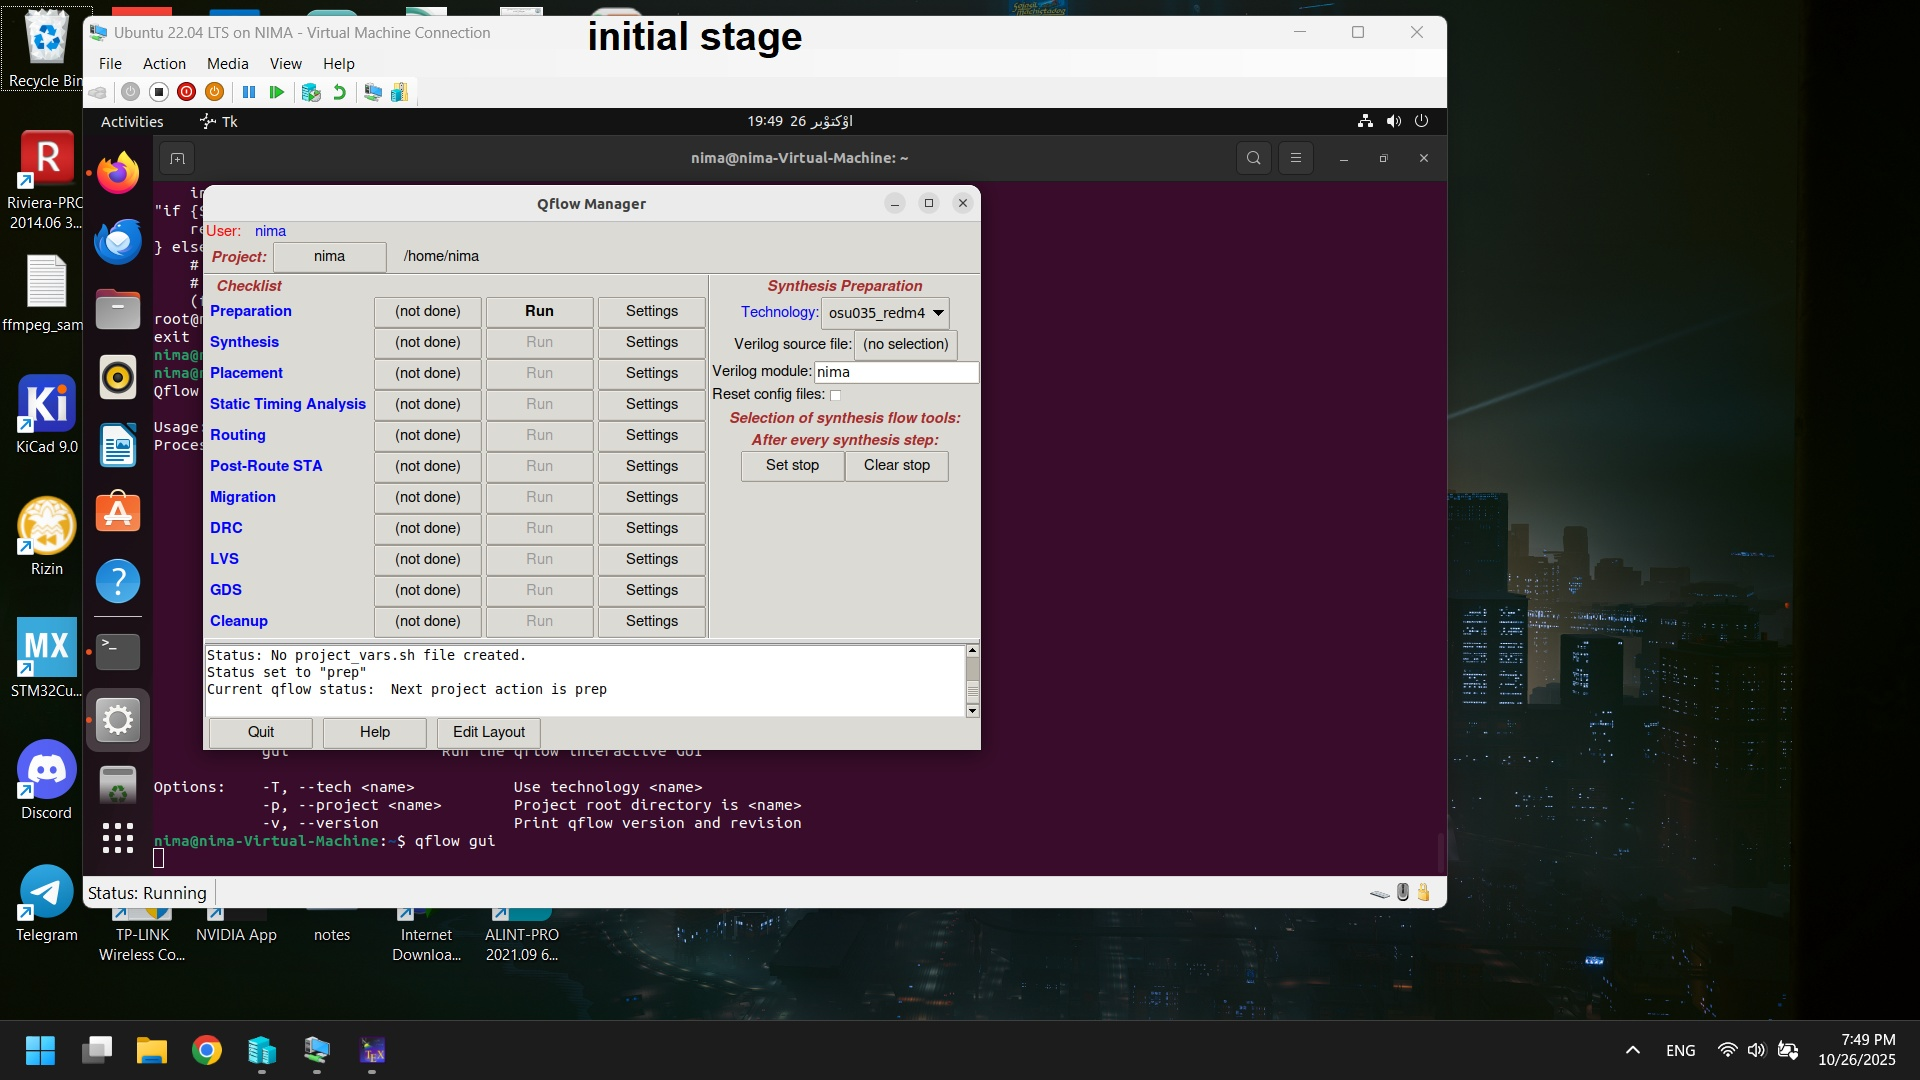
\includegraphics[scale=0.2]{init.jpg}
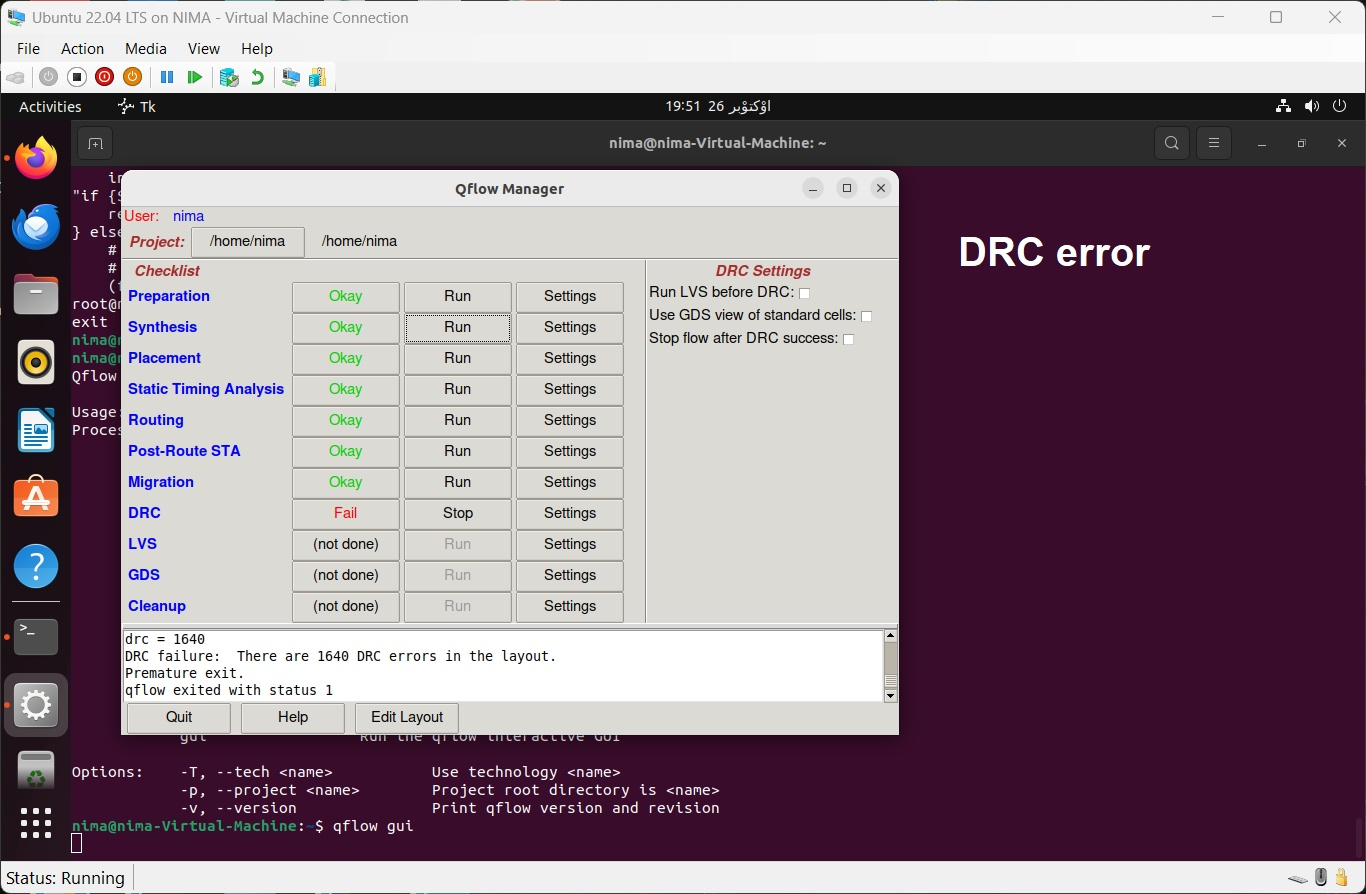
\includegraphics[scale=0.2]{drc.jpg}
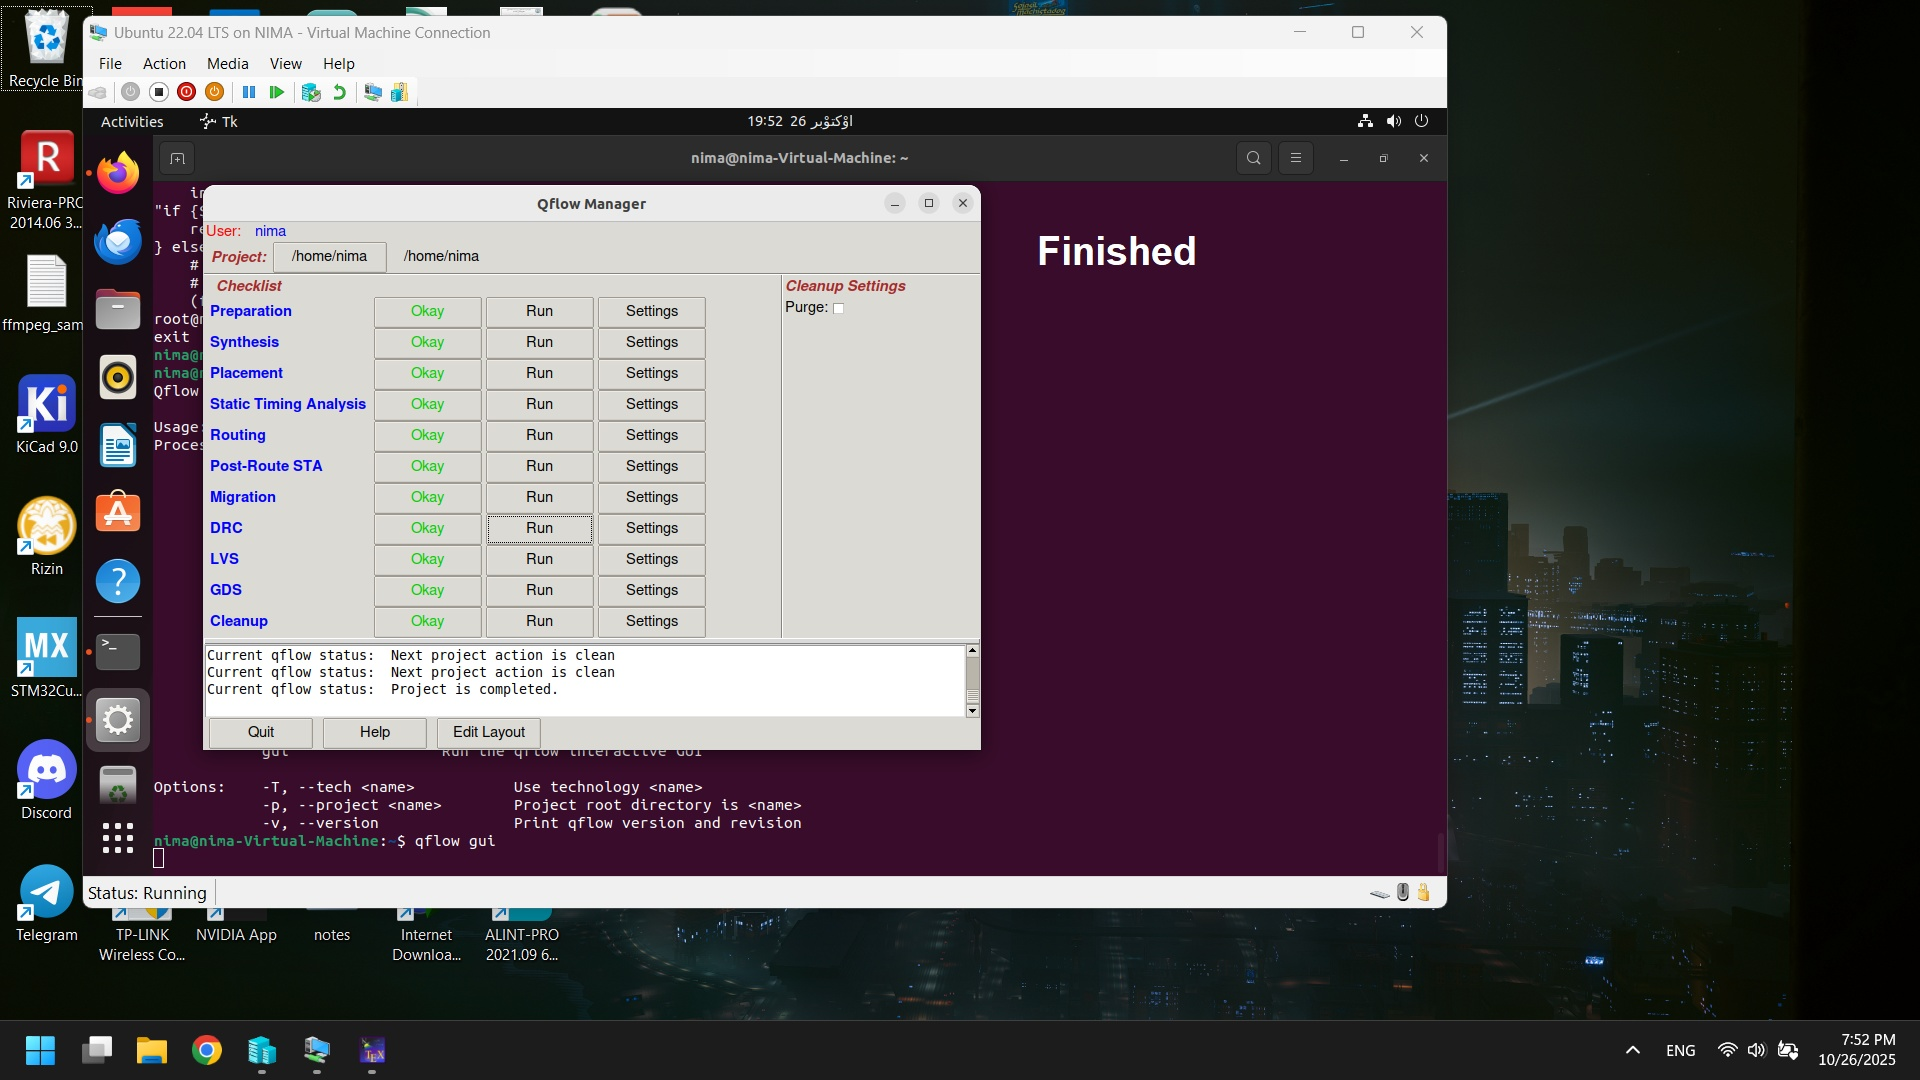
\includegraphics[scale=0.2]{finished.jpeg}
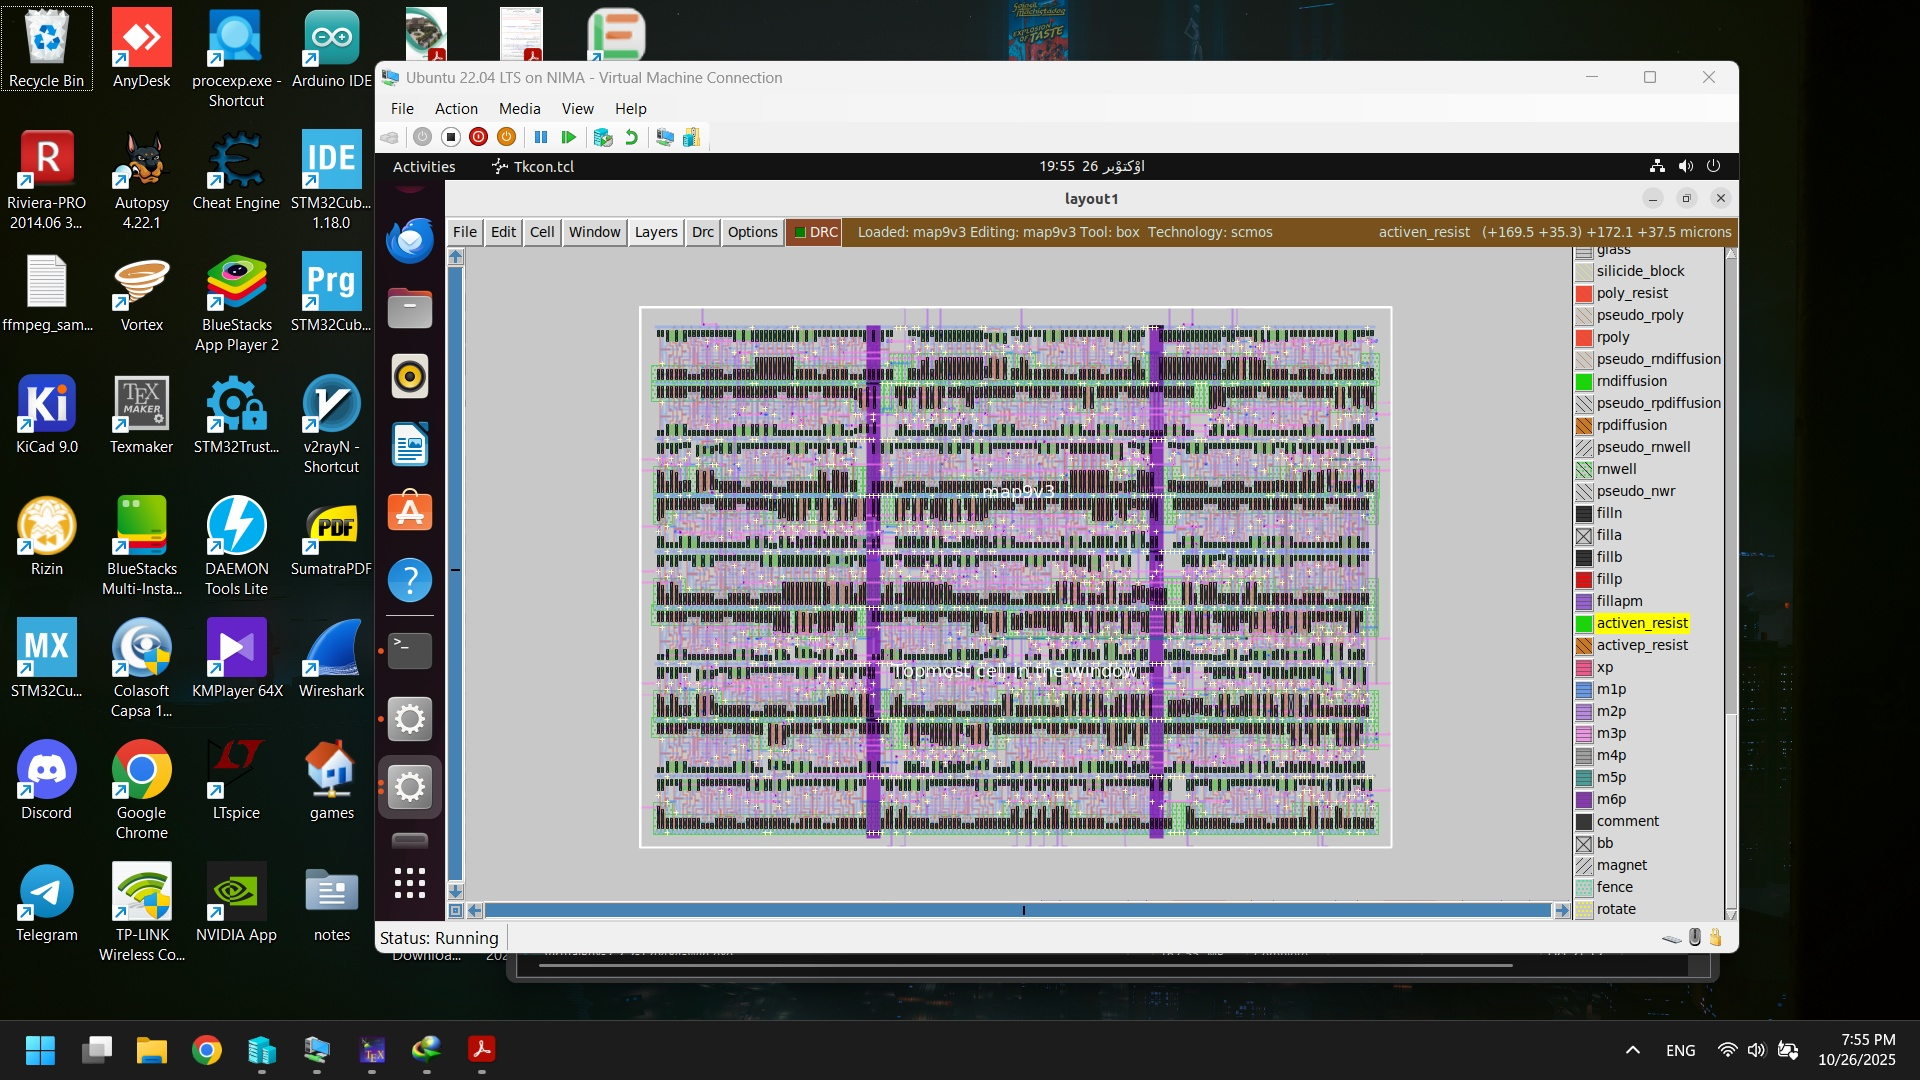
\includegraphics[scale=0.2]{layout.jpg}
\caption{QFLOW}
\end{figure}

\end{questions}


\end{document}